\documentclass[UTF8,12pt,oneside,fontset=fandol,notitlepage]{ctexart}
\usepackage[a4paper,left=2.5cm,right=2.5cm,top=2.8cm,bottom=2.8cm]{geometry}
\usepackage[dvipsnames]{xcolor}
\colorlet{accent}{MidnightBlue}
\pagestyle{plain}
\linespread{1.16}
\usepackage{titlesec}

\usepackage{amsmath,amssymb,amsthm,mathtools}
\usepackage{graphicx,booktabs,subcaption,multicol,tikz-cd}
\usepackage[version=4]{mhchem}
\usepackage{tcolorbox}


\usepackage{hyperref}
\hypersetup{colorlinks=true,linkcolor=accent,citecolor=accent,urlcolor=accent}
\newCJKfontfamily\theoremfont{FandolFang-Regular.otf}
\newtheoremstyle{mtfang}{6pt}{6pt}{\theoremfont}{0pt}
    {\normalfont\bfseries}{.}{0.5em}{}
\theoremstyle{mtfang}
\newtheorem{theorem}{定理}[section]
\newtheorem{definition}[theorem]{定义}
\newtheorem{proposition}[theorem]{命题}
\newtheorem{lemma}[theorem]{引理}
\newtheorem{corollary}[theorem]{推论}
\theoremstyle{definition}
\newtheorem{claim}[theorem]{声明}
\newtheorem{axiom}[theorem]{公理}
\setcounter{tocdepth}{1}
\setcounter{secnumdepth}{3}


% Plain mathematical environments; amsthm supplies the final QED.
\theoremstyle{definition}
\newtheorem{example}[theorem]{例}
\newtheorem{exercise}[theorem]{习题}
\renewcommand{\qedsymbol}{\ensuremath{\square}}
\newenvironment{quotationbox}{%
    \begin{tcolorbox}[colback=accent!5,colframe=accent!55,
        boxrule=.5pt]\small\kaishu
}{\end{tcolorbox}}
\newcommand{\quoteauthor}[2]{%
    \par\begin{flushright}—— #1《#2》\end{flushright}}

\begin{document}
\title{数学排版模板示例}
\author{模板示例}
\date{}
\maketitle
\section*{序言}
\addcontentsline{toc}{section}{序言}
本示例展示章节、数学环境和出版元素的排版与引用.
\newpage
\tableofcontents
\newpage

\section{层级与环境}\label{sec:env}
\subsection{数学环境}
\subsubsection{编号示例}
\begin{definition}[平方]\label{def:square}
    实数 $x$ 的平方定义为 $x^2 \coloneqq x \cdot x$.
\end{definition}
\begin{axiom}\label{ax:one}
    对每个实数 $x$, 有 $x = x$.
\end{axiom}
\begin{proposition}\label{prop:one}
    对每个实数 $x$, 有 $x + 0 = x$.
\end{proposition}
\begin{lemma}\label{lem:one}
    对每个实数 $x$, 有 $x^2 \geq 0$.
\end{lemma}
\begin{theorem}[零元的平方]\label{thm:one}
    若 $x = 0$, 则 $x^2 = 0$.
\end{theorem}
\begin{proof}
    将 $x = 0$ 代入 $x^2$, 得 $x^2 = 0$.
\end{proof}
\begin{corollary}\label{cor:one}
    若 $x = 0$, 则 $x^2 + 1 = 1$.
\end{corollary}
\begin{example}[零元]\label{ex:one}
    取 $x = 0$, 则 $x^2 = 0$.
\end{example}
\begin{exercise}[加法]\label{exercise:one}
    验证 $1 + 1 = 2$.
\end{exercise}
\begin{claim}\label{claim:one}
    数 $1$ 是正数.
\end{claim}
定义~\ref{def:square}、公理~\ref{ax:one}、命题~\ref{prop:one}、引理~\ref{lem:one}、
定理~\ref{thm:one}、推论~\ref{cor:one}、例~\ref{ex:one}、
习题~\ref{exercise:one} 和声明~\ref{claim:one} 均可跳转.


\begin{enumerate}
    \item
        先列出条件与符号.
        \begin{enumerate}
            \item
                明确对象所在的集合.
            \item
                说明映射的定义域和值域.
        \end{enumerate}
    \item
        再逐步证明结论.
\end{enumerate}
\begin{itemize}
    \item
        无序列表使用默认标记.
        \begin{itemize}
            \item
                次级条目使用另一种默认标记.
                \begin{itemize}
                    \item
                        第三级条目测试标记与缩进.
                    \item
                        第三级长条目用于检查折行后的文字是否保持对齐,
                        同时观察嵌套列表的行距与层级是否清楚.
                \end{itemize}
        \end{itemize}
    \item
        正文仍保持清晰的阅读对比度.
\end{itemize}

\section{公式与图表}
行内求和 $\sum_{i = 1}^{n} i$ 和积分 $\int_0^1 x\,\mathrm{d}x$
保持行内大小. 编号公式为
\begin{equation}\label{eq:sum}
    \sum_{i = 1}^{n} i = \frac{n(n + 1)}{2}.
\end{equation}
不编号公式为
\[
    \int_0^1 x\,\mathrm{d}x = \frac{1}{2}.
\]
长公式只在最后一行编号:
\begin{align}
    (a + b)^2 & = (a + b)(a + b) \notag \\
    & = a^2 + ab + ba + b^2 \notag \\
    & = a^2 + 2ab + b^2. \label{eq:long}
\end{align}
公式~\eqref{eq:sum} 和公式~\eqref{eq:long} 可以跳转.
行间交换图为
\[
    \begin{tikzcd}
        A \arrow[r, "f"] \arrow[d, "g"'] & B \arrow[d, "h"] \\
        C \arrow[r, "k"'] & D.
    \end{tikzcd}
\]
行内小交换图为
$\begin{tikzcd}[ampersand replacement=\&,cramped,sep=tiny]
    A \arrow[r, "f"] \& B
\end{tikzcd}$.
化学式包含可逆反应 $\ce{N2 + 3H2 <=> 2NH3}$ 和加热反应
\[
    \ce{CaCO3 ->[\Delta] CaO + CO2 ^}.
\]
这是脚注示例.\footnote{脚注内容及返回链接.}
\begin{quotationbox}
    数学的语言可以简洁地表达结构与关系.
    \quoteauthor{示例作者}{示例文集}
\end{quotationbox}
\begin{table}[htbp]
    \centering
    \caption{居中表格}\label{tab:sample}
    \begin{tabular}{cc}
        \toprule
        对象 & 数值 \\
        \midrule
        $a$ & $1$ \\
        $b$ & $2$ \\
        \bottomrule
    \end{tabular}
\end{table}
\begin{figure}[htbp]
    \centering
    
\begin{tikzpicture}
        \draw[accent,thick] (0,0) circle (0.8);
    \end{tikzpicture}
    \caption{居中图片}\label{fig:single}
\end{figure}
\begin{figure}[htbp]
    \centering
    \begin{subfigure}{0.42\textwidth}
        \centering
        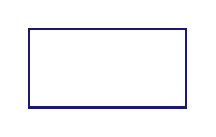
\begin{tikzpicture}\draw[accent,thick] (0,0) rectangle (2,1);\end{tikzpicture}
        \caption{矩形}\label{fig:rect}
    \end{subfigure}
    \hfill
    \begin{subfigure}{0.42\textwidth}
        \centering
        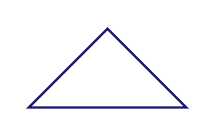
\begin{tikzpicture}\draw[accent,thick] (0,0) -- (2,0) -- (1,1) -- cycle;\end{tikzpicture}
        \caption{三角形}\label{fig:triangle}
    \end{subfigure}
    \caption{并排子图}\label{fig:pair}
\end{figure}
表~\ref{tab:sample}、图~\ref{fig:single} 和图~\ref{fig:pair}
提供交叉引用. 另见文献~\cite{sample}.

\appendix
\section{附录甲}\label{app:a}
附录 A 的正文.
\section{附录乙}\label{app:b}
附录 B 的正文.
\section{附录丙}\label{app:c}
附录 C 的正文. 参见附录~\ref{app:a}、\ref{app:b} 和~\ref{app:c}.
\cleardoublepage
\phantomsection
\addcontentsline{toc}{section}{参考文献}
\begin{thebibliography}{9}
    \bibitem{sample} 示例作者. \emph{示例文集}. 示例出版社, 2026.
\end{thebibliography}
\end{document}
